%# -*- coding: utf-8 -*-
% !TEX encoding = UTF-8 Unicode
\RequirePackage{fixltx2e}
\documentclass[aps,pre,12pt,preprint,onecolumn,showpacs,showkeys,UTF8]{revtex4-1}
\usepackage{ctex}
\usepackage{mathrsfs}
\usepackage{setspace,dcolumn}
\usepackage{subfigure}
\usepackage{graphicx,psfrag,epsfig}
\usepackage[font=small,format=plain,labelfont=bf,textfont=it,justification=raggedright,singlelinecheck=false]{caption}
\usepackage{amsmath,amsfonts,amssymb,amsthm,bm,upgreek}
\usepackage{geometry}
\usepackage[mathscr]{eucal}
\usepackage{titlesec}
\usepackage{tabularx}
\titleformat{\section}{\bf\fangsong\zihao{4}}{\thesection}{0.75em}{}
\geometry{top=2.54cm,bottom=2.54cm,left=3cm,right=3cm}
\renewcommand\appendixname{附录}
\renewcommand\abstractname{}%摘要
\renewcommand\tablename{表}
\renewcommand\figurename{图}
\makeatletter
\def\@keys@name{\songti\zihao{-4}{\bf 关键词:}}
\def\Received@name{\zihao{-5}{接收} }
\def\Revised@name{\zihao{-5}{修订} }
\def\Accepted@name{\zihao{-5}{采纳} }
\def\Published@name{\zihao{-4}{发表} }
\makeatother
\linespread{1.6}
\renewcommand{\labelenumi}{\alph{enumi}.}
\leftmargini=20mm

\begin{document}

\title{\bf\heiti\zihao{3}钠原子光谱的观测与研究\vspace{15mm}}
\author{\fangsong 乔颢\vspace{2mm}}
\affiliation{\songti\zihao{-4}北京大学物理学院2011级2班~~~~学号:1100011354 \vspace{2mm}}
\keywords{钠原子光谱, 精细结构, 能级图, 量子缺}
\email{1993422qsh@gmail.com; 18600200672}
\begin{abstract}
	\vspace{10mm}
	\begin{spacing}{1.5}
		\songti\zihao{-4}
		这个实验利用了$^{60}$Co在衰变过程中会释放出一个$\beta$粒子和两个$\gamma$光子的现象,利用$\beta-\gamma$符合测量得到了样品的绝对活度。得到的数值为$D=(5.4\pm0.2)\times10^5 min^{-1}$。理论值为$D=5.63\times10^5 min^{-1}$。实验结果与理论符合较好。
	\end{spacing}
\end{abstract}

\maketitle

\section{引言}
对元素的光谱进行研究是了解原子结构的重要途径之一。通过对于氢原子的光谱的研究,人们认识到了电子在围绕原子核运动时轨道是分立的。而对于钠原子则是一个多电子系统,对于钠原子的光谱的研究,使得人们更于清晰的了解了碱金属的电子层级结构。本实验通过对于钠原子光谱的研究,计算出钠原子价电子的量子缺,绘制出部分能级图,并且根据双线波长差计算价电子运动的时候电子实的有效电荷。

氢原子的光谱中波数可以用一下公式表示:
\begin{equation}
	\tilde{v}=\frac{R}{n_2^2}-\frac{R}{n_1^2}
\end{equation}
而对于碱原子来说,内层电子和原子核形成了原子实,所以实际上对于外层电子影响的电荷量和轨道有关。当主量子数不大的时候,这个只和角量子数有关,表述如下:
\begin{equation}
	T_{nl}=\frac{(Z_n^*)R}{n^2}=\frac{R}{(n-\Delta_l)^2}
\end{equation}

因为自旋轨道耦合,能级出现了分裂,这里也就是精细结构的出现,从理论上可以推出,对于量子数为n,l,j的能级,$j=|l\pm\frac{1}{2}|$。 有
\begin{equation}
	T_{n,l,j=l+1/2}=\frac{R}{(n'-\Delta_l')^2}-\frac{l}{2}\xi_{n,l}
\end{equation}
\begin{equation}
	T_{n,l,j=l-1/2}=\frac{R}{(n'-\Delta_l')^2}+\frac{l+1}{2}\xi_{n,l}
\end{equation}
其中有$\xi_{n,l}=\frac{R \alpha^2(Z^*)^4}{n^3l(l+1/2)(l+1)}$,所以能级分裂,波数差为:
\begin{equation}
	\Delta \tilde{v}=(l+1/2)\xi_{n,l}=\frac{R\alpha^2(Z^*)^4}{n^3l(l+1)}
\end{equation}

同时能级跃迁时候发射的光谱线强度可以由以下公式确认:
\begin{equation}
	I_{nm}=N_nA_{nm}hv_{nm}
\end{equation}
所以根据谱线跃迁的强度和定则,可以得到,对于主线系,$\frac{I_{PA}}{I_{PB}}=\frac{g_{3/2}}{g_{1/2}}=\frac{2}{1}$。锐线系有:$\frac{I_{SA}}{I_{SB}}=\frac{1}{2}$,漫线系有$\frac{I_{DA}}{I_{DB}}=\frac{1}{2}$。

这次实验通过对于钠原子光谱的探测,了解钠原子光谱的规律和其产生的原因,同时熟悉光栅光谱仪的使用。

\section{实验}
\subsection{实验装置}
\begin{enumerate}
	\item 光谱仪\ 国产WGD-8A型多功能光栅光谱仪以及其配套软件。
	\item 光源\ GY-5 钠光灯。
\end{enumerate}
\subsection{实验步骤以及数据}
打开计算机,打开仪器以及钠光灯,并对其进行预热。在系统稳定前光谱线可能不是很稳定。等到整体系统稳定后,可以进行仪器的测试以及校准。

首先将入射光阑和出射光阑都调整到合适的位置(大概不大不小),增益的负高压都调整为1,这时进行一次全谱的预扫描,来检测仪器是否正常工作。可以观测到输出的光谱强度图像在590nm左右出现极大,这也就是钠双黄线,本次实验要据此对光谱仪进行校准工作。

调整扫描范围在双黄线对应的位置,然后减少入射光强,对双黄线光谱进行详细的扫描。在光强增益调整合适的情况下测峰得到对应的钠双黄线的波长,与理论值比较后输入相对差值来校准仪器。校准过后仪器给出的波长就应该是正确的波长值。截图如下。此时测量的参数为:增益1,电压330V,负高压1,入射狭缝读数3.784mm,出射读数3.442mm。

\begin{figure}[h]
	\begin{center}
		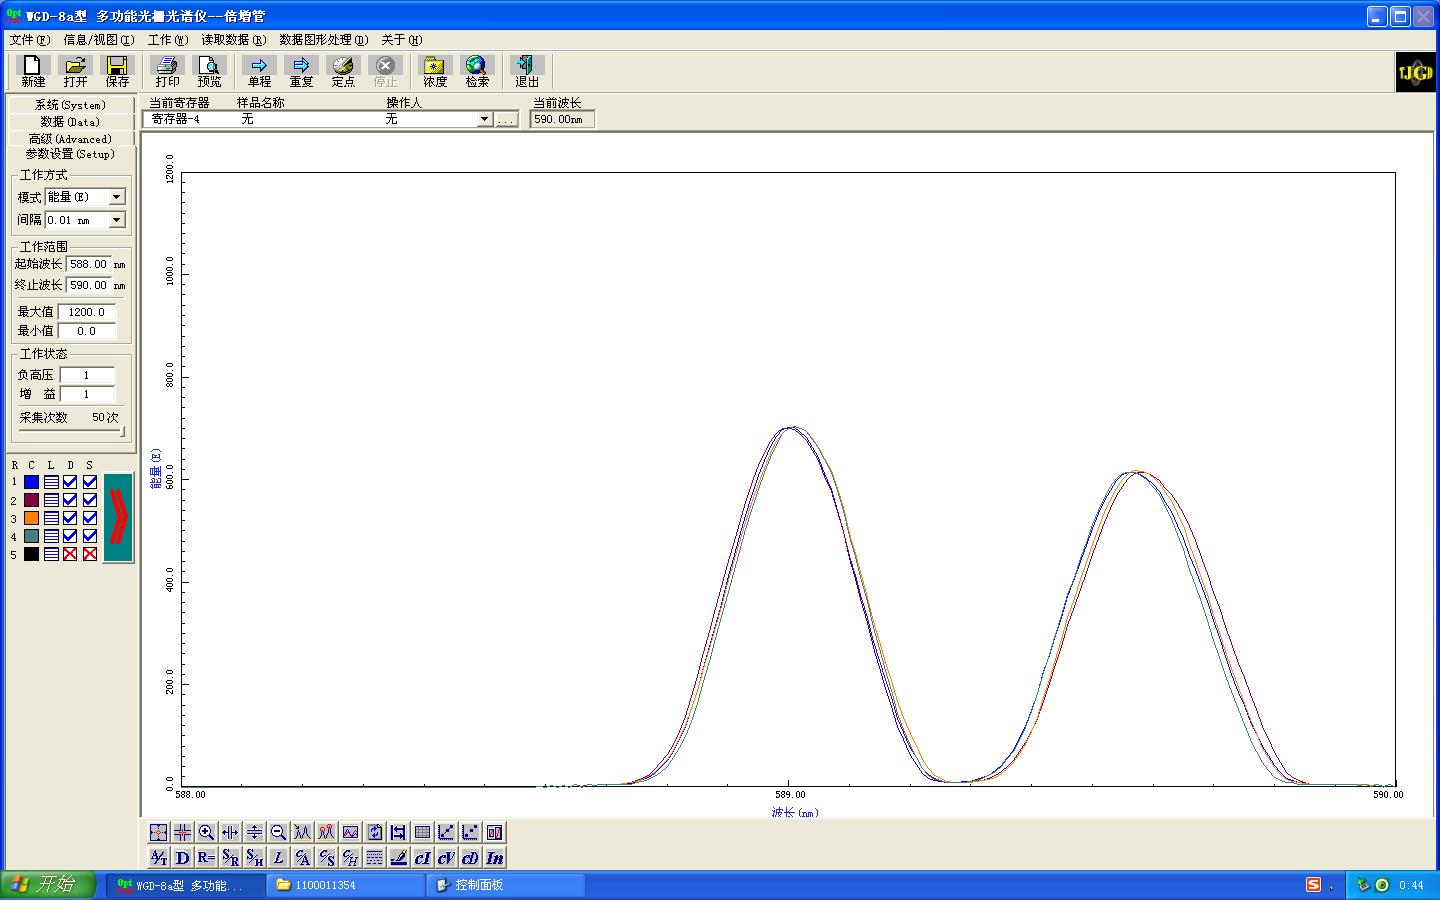
\includegraphics[width=0.7\textwidth]{pic1.png}
		\caption{\label{fig:exp1}校准后钠双黄线的强度和波长关系图}
	\end{center}
\end{figure}

\newpage

随后

\section{结论}

本实验通过$\beta-\gamma$符合测量测定$^{60}$Co的活性,得到的结果是
\begin{equation}
	D=(5.4\pm0.2)\times10^5 min^{-1}
\end{equation}
与理论之相比偏小。可能是由于参数调整的原因造成的。

\section{致谢} 
感谢楼建玲老师的指导,以及贾春燕,冉书能老师的技术支持。


\begin{thebibliography}{}
	\bibitem{Book} 吴思成,王祖铨~2010 近代物理实验(第三版)(北京:高等教育出版社)第274页.%
%
\end{thebibliography}

\clearpage
\appendix
\section{思考题}

1、实验中采用闪烁计数器,将粒子的能量吸收转化为光信号,并通过光电倍增管形成电信号,经过下游电路筛选整形等处理后计数。$\beta$计数用$\beta$探头测量值与加上铝板遮住的值的差即可。$\gamma$用样品值减去本底值即可。

2、固定一路后在示波器目测另外一路产生的信号,调整延迟从目测符合发生次数较少到最多期间即可确定出测量范围。这时候测量较快。

3、由公式可以得到要求$\tau < \frac{1}{20D}$ 即可。代入活度就可以得到分辨时间。

4、不可太厚影响$\gamma$粒子的探测,也不能太薄以至于不能完全阻挡$\beta$粒子。5mm左右是一个比较合适的值。

5、可以使用双$\gamma$测量,不过因为光子之间有一定的角度,所以可能需要矫正。有最后计算为$D=\frac{m_{1\gamma}m_{2\gamma}}{2m_{2\gamma}}$。推导过程中要用到认为放射的光子各项同性,向各个方向发射的概率是一样的。同时也要求探头的性能一致,这样才可以使得探头接收到的光子的概率相同从而能使用上述公式。

\section{记录本}
已经检查了,就不上传了。

\end{document} 
